\section{Evaluation}
\label{sec:eval}
We first give the experimental setup, then
compare and contrast the end-to-end results against various
strong baselines on three datasets,
before analyzing the main advantages of our approach.

\subsection{Datasets}
In this experiment, we use three datasets.

\textbf{Yelp} 
\footnote{\url{https://www.yelp.com/dataset}}
contains a large number of reviews about consumer services. 
Each sample in its development and test set~\cite{MeanSum19} contains 8 reviews and one corresponding human-written summary.

\textbf{Amazon} 
%\footnote{\url{https://cseweb.ucsd.edu/~jmcauley/datasets.html}}
is a dataset~\cite{HeM16} 
made up of product reviews. 
Each sample in its development set and test set has 8 reviews and 3 human-written summaries~\cite{Copycat20}. 

\textbf{RottenTomatoes} (RT) ~\cite{RT16}
%~\footnote{\url{https://web.eecs.umich.edu/~wangluxy/data.html}}
is a large set of movie reviews. Each set of reviews (on average 100) about a
movie has a human-written gold summary. 
%However, we do not use the gold summaries for training, 
%because we are targetting an unsupervised setting.

We construct the synthetic mix-structured training set for these three datasets.
Human-annotated multi-review and summary pairs
are used as development and test set
(See \tabref{tab:datasets} for detail).  
%Details are shown in \tabref{tab:datasets}.
\footnote{The size of our synthetic training set does not exceed that of previous synthetic training set.
%\JQ{remove this footnote and shown in Appendix?}
} %in \secref{sec:base}.}.

\begin{table}[th]
	\scriptsize
	\centering
	\begin{tabular}{|l|c|c|c|}
		\hline
		\textbf{} & \textbf{Training} &\textbf{Development} & \textbf{Testing}\\
		\hline
		Yelp & 100k & 100 & 100 \\
		Amazon & 90k & $28\times3$ & $32\times3$ \\
		RT & 25k& 536 & 737\\
		\hline
	\end{tabular}
	\caption{%Data statistics show 
		Dataset statistics.
	    Training column shows the number of our synthetic training pairs.
		$\times3$ means 3 manual summaries per multi-review.}
	\label{tab:datasets}
\end{table}

\subsection{Implementation Details}
%In this experiment,
%we apply aspect-guided models on transformer seq2seq model~\cite{Transformer17} and pretrained BART~\cite{BART20}.
When creating synthetic training data, 
we set $N$ (\secref{sec:gauss}) to be $8$ for Yelp and Amazon,
and $100$ for RT, because it depends on the number of input reviews in each test pair. 
Each test pair in Yelp or Amazon has 8 reviews as input. Each testing pair in RT has about 100 (on average) reviews as input. 
During training, we take synthetic OAs and ISs as mix-structured input and sampled summaries as output.
At test time, we extract OAs and ISs from multi-reviews in human-annotated test sets as mix-structured input and human-annotated summaries as output.
For transformer~\cite{Transformer17}, we use SGD as the optimizer.
The initial learning rate is $0.1$, momentum $\beta=0.1$,  
decay $\gamma=0.1$. 
%During test, the beam size is $5$.
For BART, we use {\em bart.large} model with its 
default settings and fine-tuning it~\citet{BART20} with
$lr=3e$-$05$. 
%The temperature in Eq. \ref{eq:T} is $0.2$.
The reason for choosing BART as our basic model is that BART is effective on summarization and easy to use. 
As our proposed approach is orthogonal to the seq2seq model, 
we expect our approach to benefit opinion summarization methods regardless of the seq2seq model architecture.
We train our models~\footnote{Data and code: \url{https://github.com/YizhuLiu/Opinion-Summarization}} on one RTX 2080Ti GPU with 11G RAM. 
The average training time of our approaches is about $10$ hours.

\cut{
\YZ{appendix}
Compared with other baselines, OpiDig and FewSum used different test sets in their papers.
To be fair, we apply them to the same test sets used in other methods.
As all baselines are unsupervised or weakly-supervised except for FewSum, 
we adopt the FewSum that is not fine-tuned on the human-annotated summaries.
}

\subsection{Models under Comparison}
\label{sec:base}
Different methods trained on their own synthetic training data are listed in \tabref{tab:base}.
\begin{table}[th]
	\scriptsize
	\centering
	\begin{tabular}{|p{7cm}|}
		\hline
		\textbf{MeanSum}~\cite{MeanSum19}: An autoencoder model, which decodes the summary based on the mean representation of input reviews. \\
		\hline
		\textbf{Copycat}~\cite{Copycat20}:  A hierarchical variational autoencoder model with the controlling of novelty. \\
		\hline 
		\textbf{OpiDig}~\cite{OpiDig20}: A self-training model with a review as output and the OAs of this review as input for training. \\
		%At test, it selected the important OAs from the multi-reviews and generated summaries. \\
		\hline
		\textbf{Denoise}~\cite{Denoise20}: A denoising summarization model with linguistically motivated noising datasets. \\
		\hline
		\textbf{FewSum}~\cite{Fewshot20}:  A conditional transformer model, including content coverage, writing style and length deviations. \\
		\hline
		\textbf{PlanSum}~\cite{Plansum20}: A summarization model trained on sentiment and aspect distributions of  reviews. \\
		\hline
		\textbf{TranSum}~\cite{transsum21}: A summarization model with sentiment and aspect embeddings as input. \\
		\hline 
	\end{tabular}
\cut{
	\begin{tabular}{|p{7cm}|}
	\hline
	\textbf{OURS (basic)}: Our proposed approach in \secref{sec:basicmodel}. {\bf Basic Model} is based on pretrained BART~\cite{BART20}, and Basic Model w/o pretrained is based on non-pretrained Transformer~\cite{Transformer17}. \\
	\hline
	\textbf{OM}: Our proposed optimized model in \secref{sec:optmodel}. Similar to BM, {\bf OM-T} is based on Transformer, and {\bf OM-B} is based on BART. \\
	\hline
	\end{tabular}
}
	\caption{Different opinion summarization approaches.}
	\label{tab:base}
\end{table}

Our proposed models can be based on non-pretrained Transformer~\cite{Transformer17} and 
pretrained BART~\cite{BART20}. By default, our proposed {\bf basic model (OURS$_{basic}$)} 
and {\bf optimized model (OURS)} are based on BART. 

\cut{%%
	\begin{itemize}
		\item \textbf{MeanSum}~\cite{MeanSum19} was an unsupervised auto-encoder model, which decodes the summary based on the mean representation of input reviews.
		\item \textbf{CopyCat}~\cite{Copycat20} used a hierarchical variational autoencoder model with the controlling of novelty between inputs and the generated review.
		\item \textbf{OpiDig}~\cite{OpiDig20} took a review as output and the OAs of this review as input for training. At test, it selected the important OAs from the multi-reviews
		and generated summaries.
		\item \textbf{Denoise}~\cite{Denoise20} presented a denoising summarization model with linguistically motivated noising datasets.
		\item \textbf{FewSum}~\cite{Fewshot20} was a conditional transformer model specially designed on consideration of review properties, including content coverage, writing style and length deviations.
		\item \textbf{PlanSum}~\cite{Plansum20} trained sentiment and aspect distributions for synthetic dataset construction and summary generation.
		\item \textbf{TranSum}~\cite{transsum21} trained sentiment and aspect embeddings as review embeddings and used these embeddings as input of the summarization model.
		%and computed the distance between summary and all remaining reviews as weights of review embeddings for summarization.
	\end{itemize}
	Both PlanSum and TranSum 
	need human to annotate sentiment labels
	for each review in the corpus.
	However, our approach only needs reviews without any other human-annotated labels.
}%%%

\cut{
	In the following experiments, we denote the basic aspect-guided model as {\bf BM}, 
	the advanced aspect-guided model as {\bf AM}, 
	and the training of advanced model initialized with pretrained basic model as {\bf TBA}. TBA has two variants: TBA-T which 
	stands for TBA based on non-pretrained Transformer~\cite{Transformer17}, and TBA-B which stands for TBA based on pretrained BART~\cite{BART20}
	\footnote{https://github.com/pytorch/fairseq}.
}

\subsection{Evaluation Metrics}
We show the {\em automatic metrics}
and {\em human evaluation} \footnote{The Fleiss' Kappa coefficient of judges is 0.63, indicating substantial agreement.}
below.
%\YZ{Appendix}\footnote{For the generated summary with multiple gold summaries, we compute the average of its scores (ROUGE, Div$\downarrow$ and AC) based on each gold summary. This is not suitable for human evaluation, as human takes input multi-review as reference.}.

%\textbf{Automatic Metrics.}

%\begin{itemize} 
%\item 
\textbf{ROUGE}~\cite{rouge}
%\footnote{https://github.com/andersjo/pyrouge} 
(F1) include
%is the standard evaluation metric in summarization task,
ROUGE-1 (R-1), ROUGE-2 (R-2) and
ROUGE-L (R-L). 
\footnote{
Previous methods used different toolkits,
so the ROUGE scores in some published papers cannot be compared.
To be fair, we use {\em pyrouge} (https://pypi.org/project/pyrouge).
We re-evaluate Copycat and FewSum by pyrouge,
so their results may be slightly different from 
their published versions.}

\textbf{Diversity} (Div$\downarrow$) uses self-BLEU~\cite{SelfBleu18}
~\footnote{\url{https://github.com/geek-ai/Texygen}}
which measures BLEU scores of each generated sentence by considering others as reference. 
The lower value means more diversity.

\textbf{Aspect Coverage} (AC) measures the overlapping of aspects in the gold summary and generated summary.
We ask $3$ annotators to extract aspects from text. 
Given a generated summary and its gold summary,
annotators manually extract aspects from them.
We take aspects of gold summary as reference,
and compute R-1 recall between the reference  
and aspects of generated summaries.
%\footnote{We showed them some examples similar to the review in Table 1 and told them that the words, like food, service and experience, are aspects. }
%AC is the average of these R-1 recall scores.
%\end{itemize}

\textbf{Human Evaluation.}
We randomly select 50, 32 (all test data) and 50 samples 
from the test sets of Yelp, Amazon and RT, respectively. 
We ask three 
human annotators,
who are native or proficient English speakers to 
rank gold summary and summaries 
generated by OURS and TranSum under 5 aspects:
{\em Fluency} (Flu.), {\em Non-redundancy} (NR.), {\em Opinion Consistency} (Cons.) and {\em Overall}.
\cut{
\YZ{Appendix}
{\em Fluency} (Flu.): the summary is grammatically correct and easy to understand; {\em Coherence} (Coh.): the summary is well organized; {\em Non-redundancy} (NR.): there is no unnecessary repetition; {\em Opinion Consistency} (Cons.): the summary reflects common opinions expressed in reviews; {\em Overall}: select the best and the worst summary on your own criteria.
}
\citet{bestworst16} show that Best-Worst Scaling~\cite{bestworst} is more reliable.
Thus, we apply Best-Worst Scaling on individual aspects, which computes the percentage of times a model was selected as the best minus the percentage of times it was selected as the worst.
%\footnote{We show annotators each multi-review and its corresponding summaries generated by different approaches. We shuffled the summaries and masked their generation methods.}

\begin{table*}[t]
	\centering
	\scriptsize
	\begin{tabular}{|l|m{0.45cm}<{\centering}m{0.45cm}<{\centering}m{0.45cm}<{\centering}cc|m{0.45cm}<{\centering}m{0.45cm}<{\centering}m{0.45cm}<{\centering}cc|m{0.45cm}<{\centering}m{0.45cm}<{\centering}m{0.45cm}<{\centering}cc|}
		\hline
		\multirow{2}{*}{\bf Approach} & \multicolumn{5}{c|}{\bf Yelp} &  \multicolumn{5}{c|}{\bf Amazon} & \multicolumn{5}{c|}{\bf RT} \\ \cline{2-16}
		& R-1 & R-2 & R-L& AC &Div$\downarrow$ & R-1 & R-2 & R-L& AC & Div$\downarrow$ & R-1 & R-2 & R-L& AC & Div$\downarrow$\\
		\hline
		Meansum & 28.86 & 3.66 & 15.19 & 0.34 & 0.38 &  29.20 &4.70 & 18.15& 0.17& 0.40 & 15.79 & 1.91 & 12.26 & 0.13 & 0.28 \\
		Copycat & 29.47 & 5.26 &18.09& 0.38 & 0.34 & 31.97 & 5.81 &20.16  & 0.18 & 0.43 & 14.98 & 3.07 & 12.19 & 0.13 & 0.28 \\
		OpiDig & 29.96 &5.00 & 17.33& 0.39 & 0.33 & 29.02 & 5.14 & 17.73 & 0.23 & 0.32 & 14.21 & 1.82& 10.23 & 0.15& 0.27 \\
		Denoise & 30.14 & 4.99 & 17.65& 0.39 & 0.27 &31.76 & 5.85 & 19.87 & 0.22 & 0.27 & 21.26 & 4.61& 16.27& 0.16& 0.25 \\
		FewSum
		& 31.96 & 5.64 & 17.77 & 0.38 & 0.28 & 32.04 & 5.93 & 20.03 & 0.20 & 0.30& 20.44& 4.79& 16.12 & 0.15& 0.26\\
		OURS w/o PLM & 33.43 & 6.27 & 18.37& 0.41 & 0.22 & 32.57 & 6.19 & 20.18 & 0.33 & 0.26& 21.56&5.23 & 17.00& 0.17& 0.24\\
		\hline
		PlanSum & 34.79&7.01 &19.74 &0.40 & 0.26 & 32.87 &6.12 & 19.05 & 0.23 & 0.32 & 21.77& 6.18 & 16.98 & 0.16 & 0.24 \\
		TranSum & 36.62&8.41 &20.31 &0.38 & 0.27 & 34.23& 7.24 & 20.49 & 0.23 & 0.32 & 25.34& 8.62& 18.35& 0.16 & 0.25\\
		OURS & \underline{\bf 36.78} & \underline{\bf 8.66} & \underline{\bf 20.52} &  \underline{\bf 0.44} &  \underline{\bf 0.20} & \underline{\bf 34.50} & \underline{\bf 7.64} & \underline{\bf 20.73} &  \underline{\bf 0.34} &  \underline{\bf 0.25} & \underline{\bf 25.44}& \underline{\bf 8.75}& \underline{\bf 18.52}& \bf 0.17&  \underline{\bf 0.23}\\
		\hline
	\end{tabular}
	\caption{Automatic evaluation. 
		%OURS w/o pretrain is OURS using non-pretrained transformer.
		%TBA-T and TBA-B are based on Transformer \cite{Transformer17} and BART \cite{BART20} respectively.
		The scores underlined are significantly better than TranSum (p$<$0.05). 
		``PLM'' means  pretrained language model. %\JQ{explain why approaches are separated into two parts}
		%\footnotesize{The ROUGE scores of OpiDig and FewSum are different from the published version because their test sets are different from other approach. To be fair, we select the test sets used in most approaches.} 
	}\label{tab:all}  
\end{table*}

\subsection{Main Results}
\label{sec:results}
%\tabref{tab:all} compares our best model OURS with previous methods.
As shown in \tabref{tab:all} ,
among all the models that don't use any pretrained language model, 
OURS w/o PLM performs the best.
Compared with TranSum and PlanSum, the ROUGE scores of OURS is lower
because TranSum and PlanSum introduce external knowledge by using pretrained BERT~\cite{BERT19}.
OURS using pretrained BART achieves the best scores in terms of ROUGE, AC and Div$\downarrow$,
demonstrating the full strength of our created synthetic training data.
In general, our approaches receive higher AC scores but lower Div scores since the model benefits 
from directly taking OAs as input and captures complementary information from ISs. The summary generated by OURS in \tabref{tab:overall_exp} contains more implicit information, such as ``patio seating''.
%\KZ{More diversity because of the IS? can u be a bit more specific here?} 
Compared to Amazon, the advantage of our best model on Yelp is less
because each sample has 3 gold summaries in Amazon and has only one gold summary in Yelp.
%\KZ{I don't quite understand the logic here: 
%Since a single gold summary covers less information than multiple gold summaries,
The improved generated summaries are more likely to match tokens in multiple gold summaries. 
Thus, even if the generated summary on yelp covers more important information, the rouge score may not change much.

\cut{
\YZ{Limitation}
\begin{table}[th]
	\begin{center}
		\scriptsize
		\subtable[Yelp]{
		\begin{tabular}{|l|m{5.8cm}|}	
			%\hline \bf{BAG} \\
			\hline
			Gold & 
			the \textbf{servers} are kind and knowledgeable . \textit{they will
			patiently answer your questions . they offer \textbf{patio seating} .}
			%\textit{seating if you ' d prefer to sit outside .} 
			the free \textbf{chips} and \textbf{salsa} are always a plus , and the \textbf{margaritas} are \textbf{amazing} too . the menu is full tasty \textbf{authentic mexican food .} \\
			\hline
			\hline
			OpiDig & a pretty \textbf{place} . the \textbf{service} is amazing and the \textbf{food} is amazing . 
			\color{red}{\textbf{atmosphere} is great and the \textbf{portions} are huge}
			%\vspace{0.25em}
			\\
			\hline
			TranSum& i love this \textbf{place} . the \textbf{food} is good and the \textbf{service} is great . the \textbf{chips} and \textbf{salsa platter} is huge enough. 
			\textit{\color{red}{the only thing is that it 's a little pricey for what you get .}}
			%\vspace{0.25em}
			\\
			\hline
			\hline
			BM & the \textbf{servers} are always \textbf{friendly} and the \textbf{food} is \textbf{great} . it is a \textbf{good mexican restaurant .} \\
			%\hline \bf{BAI} \\
			\hline
			AM & \textbf{great food} , \textbf{great service} , \textbf{great atmosphere} , and \textbf{great prices} . \color{red}{i have been there a few times and have \textbf{never} had a \textbf{bad experience} . }
			\vspace{0.15em}
			\\
			\hline
			TBA & it 's one of the \textbf{authentic mexican restaurant} in the area. the \textbf{food} is great . the \textbf{servers} are very friendly and knowledgeable . \textit{they took the order patiently .} the \textbf{chips} and \textbf{salsa} are good too . \textit{it is huge and has \textbf{patio seating} . } 
			%\color{gray}{you can get a lot of food for the price you pay . }
			\\
			\hline
		\end{tabular}
	\label{tab:expy}
	}
\qquad
\subtable[RT]{
		\label{tab:exprt}
			\begin{tabular}{|l|m{5.8cm}|}	
		%\hline \bf{BAG} \\
		\hline
		Gold & 
		\textit{\textbf{movie} begins with promise .}
		but it suffers from a flimsy \textbf{narrative} and poor \textbf{execution} . \textit{with alien-sized plot holes} \\
		\hline
		\hline
		OpiDig & \color{red}{great \textbf{concept} . a strange but cool \textbf{comedy} .}
		\\
		\hline
		TranSum& \textbf{hancock} is a \textbf{movie} that's a lot of fun, \color{red}{but it'll be a bit of the same time as the \textbf{movie}.}
		%\vspace{0.25em}
		\\
		\hline
		\hline
		BM & \textcolor{red}{great \textbf{concept}} , shaky \textbf{narrative} .  \textcolor{red}{\textbf{hancock} is a strange and fun \textbf{film} .} \\
		\hline
		AM & \textbf{hancock} has a promising premise ,
		but the \textbf{narrative} slips into a confusing \textbf{backstory} . \\
		\hline
		TBA & \textbf{hancock} has a promising premise ,
		but the \textbf{narrative} slips into a confusing \textbf{backstory} . 
		\\
		\hline
	\end{tabular}
}
	\end{center}

	\caption{Summaries generated by different models and their gold summary. Bolded words are aspects. The sentences in red don't match Gold summary. The italicized sentences are ISs. BM, AM and TBA are based on BART.
	}			\label{tab:overall_exp}  
\end{table}
}
%\KZ{you are still missing a lot of necessary ``the'' and ``a'' everywhere. Check carefully throughout the paper.
%Also consider breaking long paras to smaller ones.}
\tabref{tab:overall_exp} compares the summaries generated by the best models trained on 
structured data (OpiDig), textual data (TranSum) and mix-structured data (OURS).
OpiDig clusters OAs of multi-review and then uses the center pairs to construct summaries, which may be weakened by the noise of clustering.
As shown in \tabref{tab:overall_exp}, ``atmosphere'' and ``portions'' of OpiDig's summary are not in gold summary.
Moreover, it is difficult to generate summary sentences without OAs, such as the italicized sentences in gold summary.  
Compared with OpiDig,
OURS trained on mix-structured data learns to expand important OAs
as sentences with explicit opinions and summarize ISs for implicit opinions,
which can cover more gold aspects and generate similar implicit sentences to gold summary.
For TranSum, as certain information in sampled summary cannot be found from the synthetic textual inputs during training, the summaries generated by TranSum may lose important information and contain redundant information, such as ``margaritas'' in gold summary and
the italicized sentence about ``price''.
OURS avoids the above problems because of the fine-grained 
synthetic input for the sampled summary.
Since the cost of writing opinion summaries for multi-reviews is very high, 
the size of test sets is small. The improvement of our proposed approach on all three different testing sets shows that our results are reliable. 

\begin{table}[th]
	\begin{center}
		\scriptsize
		\begin{tabular}{|p{0.75cm}|m{6cm}|}	
			%\hline \bf{BAG} \\
			\hline
			Gold & 
			the \textbf{servers} are kind and knowledgeable . \textit{they will
				patiently answer your questions . they offer \textbf{patio seating} .}
			%\textit{seating if you ' d prefer to sit outside .} 
			the free \textbf{chips} and \textbf{salsa} are always a plus , and the \textbf{margaritas} are \textbf{amazing} too . the menu is full tasty \textbf{authentic mexican food.} \\
			\hline
			\hline
			OpiDig & a pretty \textbf{place} . the \textbf{service} is amazing and the \textbf{food} is amazing . 
			\color{red}{\textbf{atmosphere} is great and the \textbf{portions} are huge}
			%\vspace{0.25em}
			\\
			\hline
			TranSum& i love this \textbf{place} . the \textbf{food} is good and the \textbf{service} is great . the \textbf{chips} and \textbf{salsa platter} is huge enough. 
			\textit{\color{red}{the only thing is that it 's a little pricey for what you get .}}
			%\vspace{0.25em}
			\\
			\hline
			%\hline
			%BM & the \textbf{servers} are always \textbf{friendly} and the \textbf{food} is \textbf{great} . it is a \textbf{good mexican restaurant .} \\
			%\hline \bf{BAI} \\
			%\hline
			%AM & \textbf{great food} , \textbf{great service} , \textbf{great atmosphere} , and \textbf{great prices} . \color{red}{i have been there a few times and have \textbf{never} had a \textbf{bad experience} . }
			%\vspace{0.15em}
			%\\
			\hline
			OURS & it 's one of the \textbf{authentic mexican restaurant} in the area. the \textbf{food} is great . the \textbf{servers} are very friendly and knowledgeable . \textit{they took the order patiently .} the \textbf{chips} and \textbf{salsa} are good too . \textit{it is huge and has \textbf{patio seating} . } 
			%\color{gray}{you can get a lot of food for the price you pay . }
			\\
			\hline
		\end{tabular}
	\end{center}
	
	\caption{Generated summaries and their gold summary from Yelp. Bolded words are aspects. The sentences in red don't match Gold summary. The italicized sentences are ISs. %TBA is based on BART.
	}			\label{tab:overall_exp}  
\end{table}


\cut{
\YZ{Limitation}
Our model achieves the best among all for RT, though the margin here becomes even less.
This is because the summaries in RT are shorter with fewer explicit OAs.
%, like Gold in \tabref{tab:overall_exp}(b).
The average number of tokens in reviews of Yelp and Amazon is about $65$, whereas that of RT is about $25$.
Movie reviews include the discussion on plots, such as italicized sentences of Gold in \tabref{tab:overall_exp}(b),
which makes the proportion of OAs in movie reviews less than that of Yelp and Amazon.
As shown in \tabref{tab:overall_exp}(b), even though the summary generated by TBA represents more information of gold summary than other baselines,
it is not much closer to gold summary. 
Therefore, the gain of our proposed TBA on RT is less than the other two datasets.
}


%We use human evaluation
%to help automatic evaluation.
In human evaluation, we assess summaries generated by the previous state-of-the-art model (TranSum), our best model (OURS) and gold summaries.
Gold gets best manual score in \tabref{tab:human}
since the gold summaries are written by human.
%The score of our model lower than PlanSum
%denotes that 
%human-annotators thinks that
The summaries generated by our model 
are better than TranSum from all perspectives.
\begin{table}[th]
	\centering
	\scriptsize
	\begin{tabular}{|l|l|ccccc|}
		\hline
		\bf Data & \bf Model & \bf Flu & \bf Coh & \bf NR & \bf Cons & \bf Overall \\
		\hline
		\multirow{3}{*}{Yelp}&Gold& 0.34 & 0.49 & 0.41 & 0.35 & 0.31 \\
		&TranSum& -0.46 & -0.53 & -0.70& -0.64& -0.48 \\
		&OURS & 0.12 & 0.14 & 0.29 & 0.29 & 0.17 \\
		\hline
		\multirow{3}{*}{Amazon}&Gold& 0.32 & 0.55 & 0.38& 0.44 & 0.32\\
		&TranSum& -0.54 & -0.67 & -0.68 &-0.72 & -0.41 \\
		&OURS & 0.22 & 0.12 & 0.30 & 0.28 & 0.09 \\
		\hline
		\multirow{3}{*}{RT}&Gold& 0.42 & 0.36 & 0.51 & 0.29 & 0.45 \\
		&TranSum& -0.61 & -0.64 & -0.66 &-0.46 & -0.48 \\
		&OURS & 0.19 & 0.28 & 0.15 & 0.17 &  0.05 \\
		\hline
	\end{tabular}
	\caption{Human evaluation. }
	\label{tab:human}
\end{table}

\subsection{Mix-structured vs. Structured or Unstructured Synthetic Data}
\label{sec:per}
To evaluate the effectiveness of mix-structured data versus
other kinds of synthetic data,
we convert structured and non-structured synthetic input into mix-structured version, and compare previous approaches trained on their original synthetic data
and OURS$_{basic}$ trained on the mix-structured version of previous synthetic data.
This is the best way to compare data in different types,
as different synthetic datasets must be accompanied by their compatible models.
Results are shown in 
\figref{fig:abl_data}.%\tabref{tab:traindata}.

\begin{figure}[ht]
	\subfigure[Yelp]{
		\label{fig:dy}
		%\begin{minipage}[t]{0.33textwidth}
		\centering
		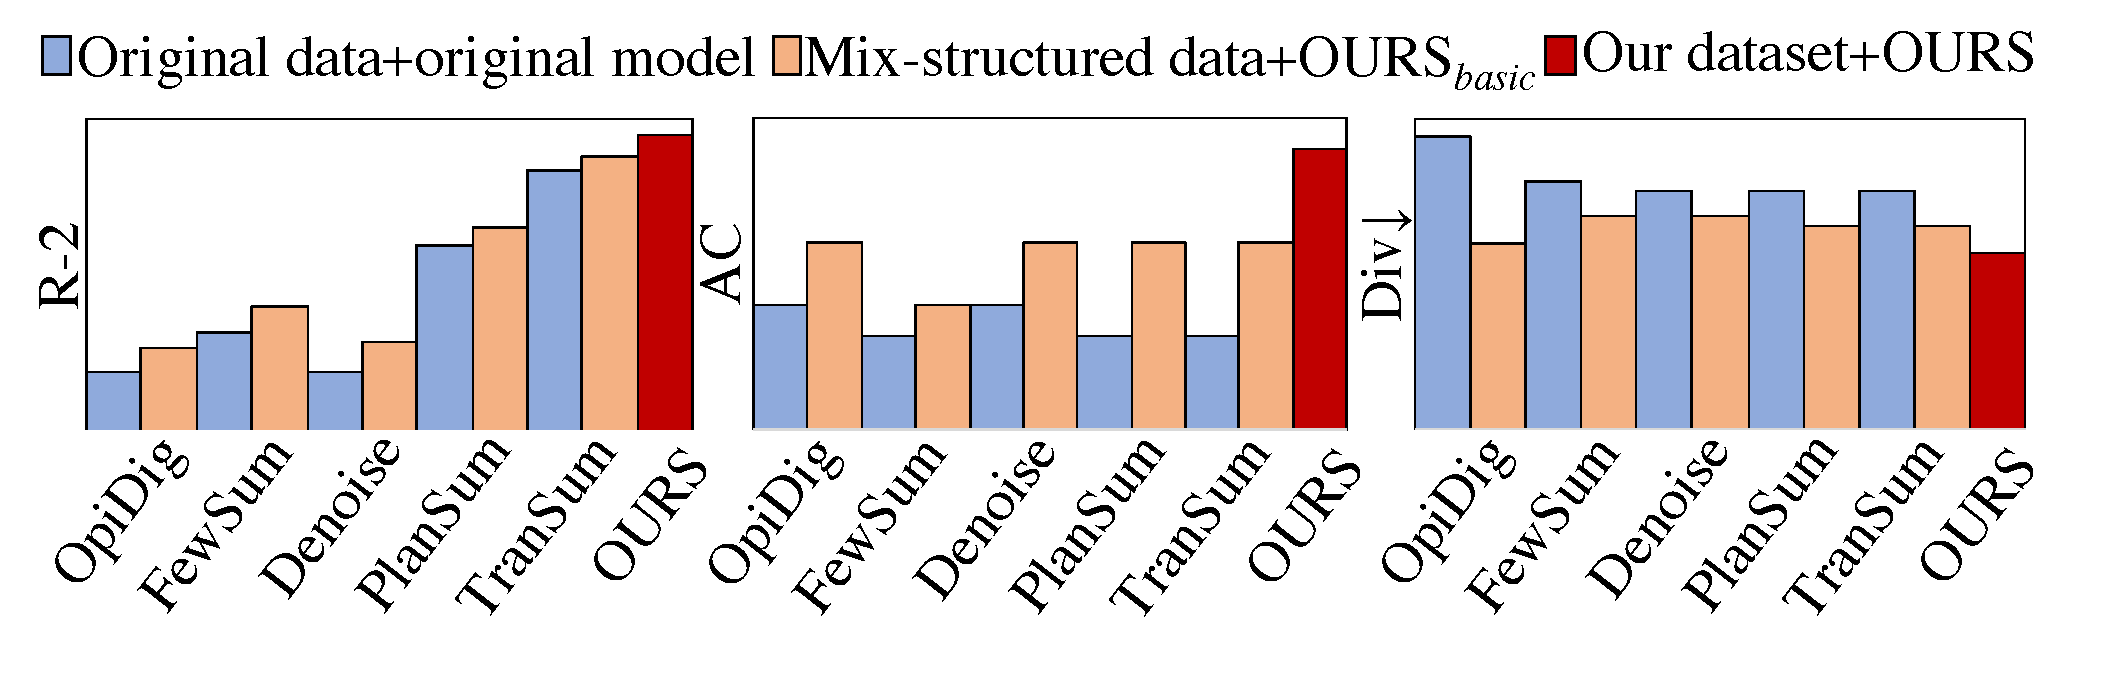
\includegraphics[width=1\linewidth]{ABL_data_Yelp.pdf}
		%\end{minipage}
	}
	\subfigure[Amazon]{
		\label{fig:da}
		%\begin{minipage}[t]{0.33textwidth}
		\centering
		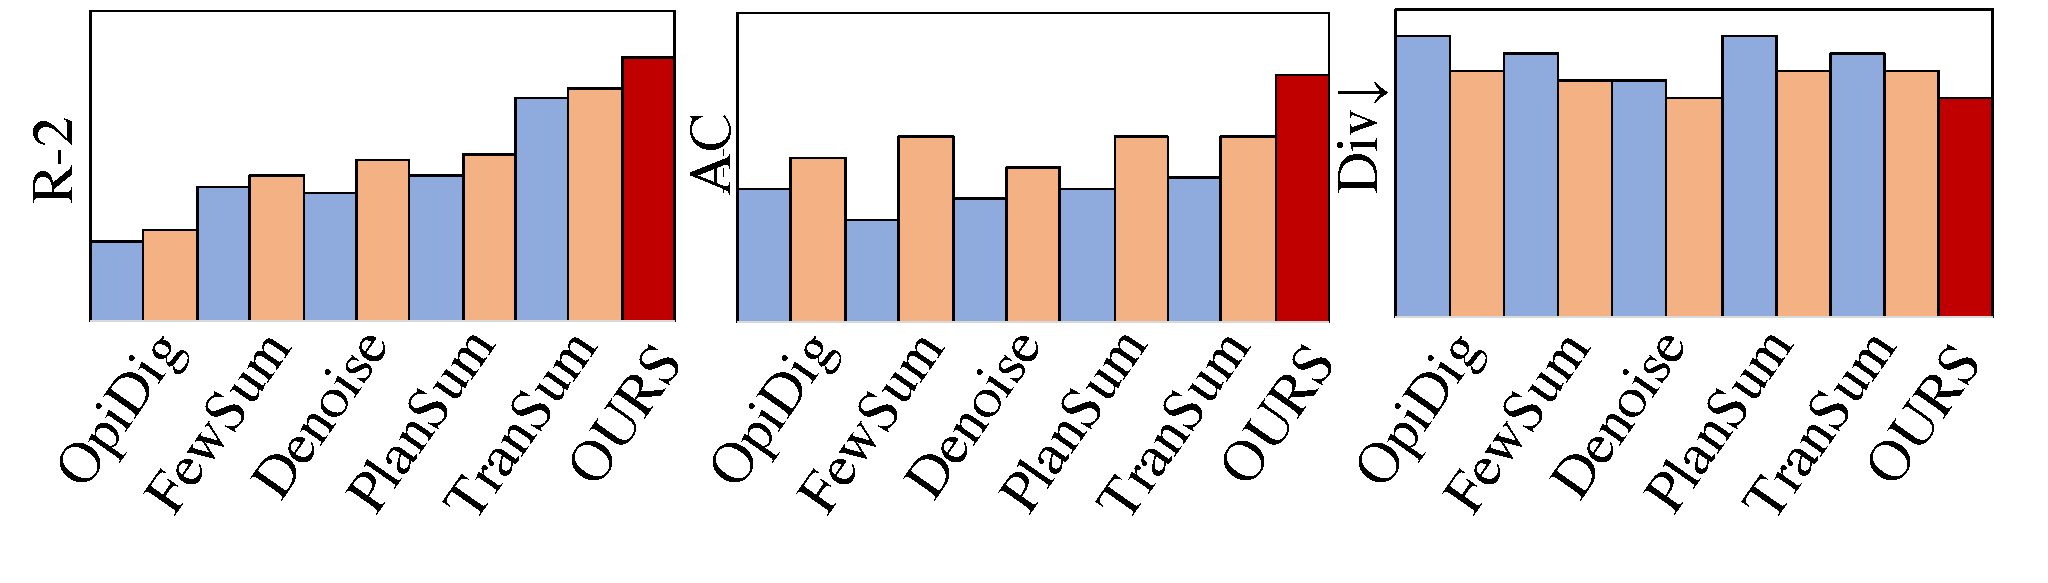
\includegraphics[width=1\linewidth]{ABL_data_Amazon.pdf}
		%\end{minipage}
	}
	\subfigure[RT]{
		\label{fig:dr}
		%\begin{minipage}[t]{0.33textwidth}
		\centering
		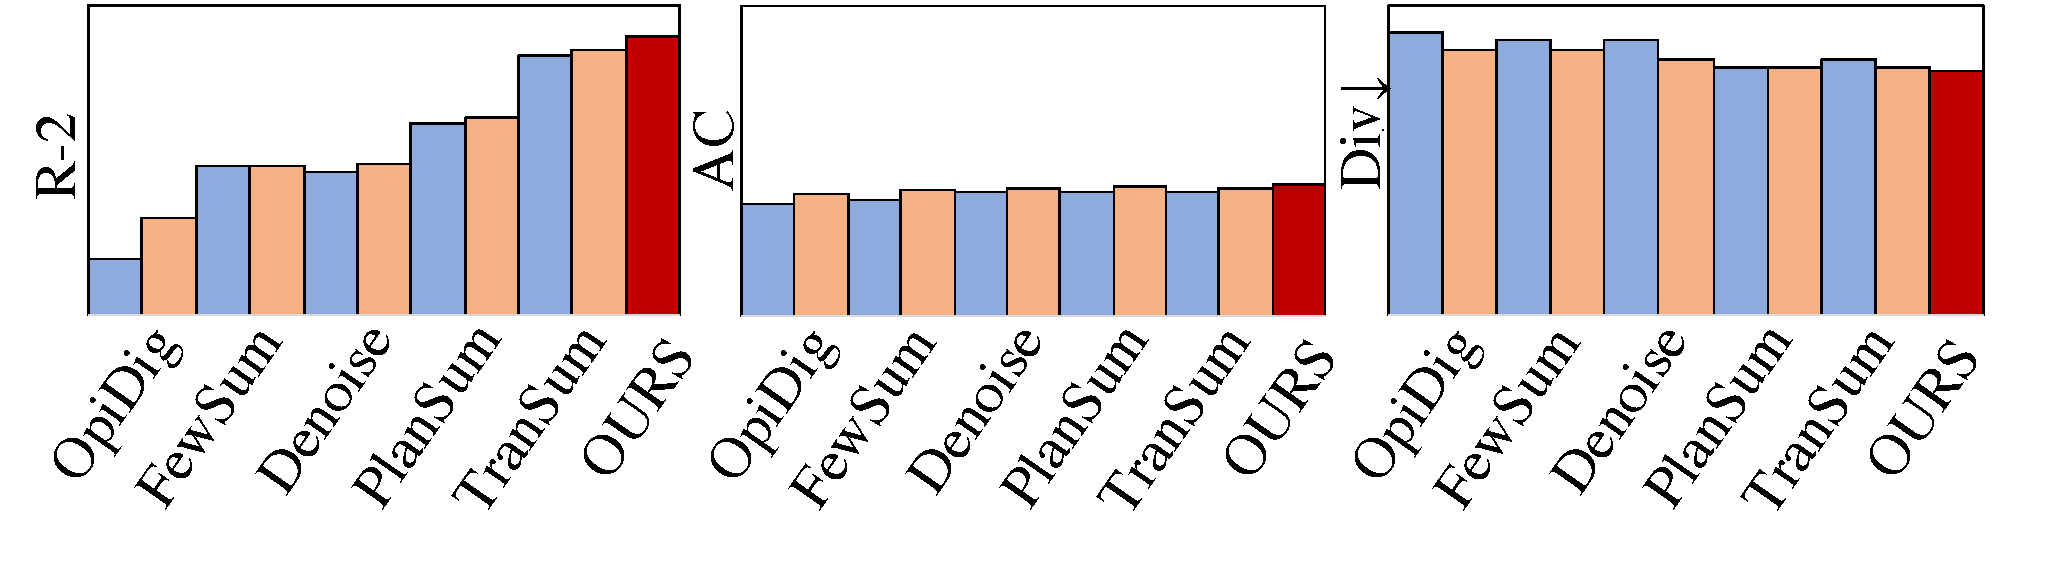
\includegraphics[width=1\linewidth]{ABL_data_RT.pdf}
		%\end{minipage}
	}
	\caption{Results on different synthetic data and their applicable models. Datasets in mix-structured version (``mix-'') use OURS model for training.%because of the characteristics of mix-structured data. 
		%\YZ{change to mixture}
		%``mix-'' means mix-structured version. 
		%The data of TransSum is from {\em leave-one-out}. OURs denotes TBA-B trained on our created mixture synthetic data.
	}
	\label{fig:abl_data}
\end{figure}

%According to different original synthetic datasets, we adopt different models for training.
%This is because a synthetic dataset must be accompanied by its compatible model.
For datasets with textual multi-review as input (FewSum, Denoise, PlanSum and TranSum), 
we convert them into mix-structured versions by extracting 
OAs and ISs
from their multi-reviews as input.
For synthetic data with structured input (OpiDig),
we construct its mix-structured version
by sampling OAs and ISs for each output in original dataset through our data creation method and taking them as input.
To be fair, for OpiDig, FewSum and Denoise,
the training on their original textual datasets did not use any pretrained language model,
so we train OURS without pretrained language models on their datasets in mix-structured version.
For mix-structured version data of PlanSum and TranSum,
we train OURS with pretrained language model on them,
as PlanSam and TranSum trained on original textual data used pretrained language model to import external knowledge.
In \figref{fig:abl_data},
OURS$_{basic}$ trained on the mix-structured version of previous textual synthetic datasets
is better than previous approaches in terms of R-2, AC and Div$\downarrow$ scores,
showing that mix-structured data
is helpful in highlighting the aspects and opinions.
Compared with the structured datasets OpiDig, the mix-OpiDig get better ROUGE scores and Div$\downarrow$ scores as the ISs in mix-structured data help the model capture implicit information.

As shown in \figref{fig:abl_data}, OURS trained on our dataset performs best since we sample OAs and ISs from all reviews except summaries and use optimized model for training,
which makes the best use of mix-structured data.

%{\em Mix-structured data.} 
%\KZ{I think this whole para incl the table can go into the beginning of \secref{sec:per}, 
%	because these are really
%	prelim study that motivate our design to do mix-structured data? And then the second part of
%	\secref{sec:per} shows the results of using mix vs. unstructured or structured alone.
%	The rest of this section is just about sampling, so u can change the section name as such.} 
To explain the rationality of mix-structured data, we call the sentences that do include OAs as \textit{explicit sentences} (ES).
We remove OAs and stopwords from ESs and compute the percentage of the remaining tokens 
in original ESs. These percentages are $10.7\%$ in Yelp, $11.1\%$ in Amazon, and $4.3\%$ in RT.
We also randomly sample 100 reviews from each dataset and ask human annotators to pick the
sentences that still contain useful information after removing OAs.
Result shows that $<10\%$ of ESs contain useful residual information, i.e., $9.1\%$ (Yelp), $9.3\%$ (Amazon), $4.0\%$ (RT).
The above results show that ESs contain very little implicit information.
Therefore, we take extract OAs from reviews as part of the input is reasonable.
Meanwhile, we calculate the distribution of ESs and ISs in multi-reviews and reference summaries in human-annotated test sets.
%Only using OAs as input will miss out the much information of multi-review
As shown in \tabref{tab:OAIS}, the proportion of ISs in multi-review and reference summary is more than $30\%$, which means that
%More than $30\%$ of sentences in reference summary are ISs, which should be summarized from the ISs in multi-review.
adding ISs is important and necessary.
\begin{table}[th]
	\scriptsize
	\centering
	\begin{tabular}{|l|cc|cc|}
		\hline
		\multirow{2}{*}{Dataset}&\multicolumn{2}{c|}{\textbf{Multi-review}}&\multicolumn{2}{c|}{\textbf{Reference summary}} \\ \cline{2-5}
		&ESs & ISs & ESs & ISs \\
		\hline
		Yelp & 0.54& 0.46&0.68 &0.32\\
		%\hline
		Amazon &  0.55&0.45&0.63&0.37\\
		%\hline
		RT &  0.33&0.67&0.32&0.68\\
		\hline
	\end{tabular}
	\caption{Proportion of ES and IS in test sets.}
	\label{tab:OAIS}
\end{table}


\subsection{Ablation}
\label{sec:abl}
We use various ablation studies on our synthetic dataset and proposed models.
%which assesses the effectiveness of our proposed approaches. 
We report R-2, AC and Div$\downarrow$ scores on test sets. 
%R-2 is the most popular of the ROUGE family, 
%which reflects the coverage of words and the consistency of word order between generated summary and its reference.
\cut{%%%%%%
\begin{table*}[th]
	\begin{center}
		\small
		\begin{tabular}{|r|c|c|c|c|c|c|c|c|c|c|c|}
			\hline
			\multicolumn{2}{|c|}{\bf Approach} & \multicolumn{5}{c|}{\bf Yelp} &  \multicolumn{5}{c|}{\bf Amazon} \\ %\cline{1-12}	
			\hline
			\textbf{Synthetic data} & \textbf{Model} & R-1 & R-2 & R-L & AC & Div & R-1 & R-2 & R-L & AC & Div \\ 
			\hline
			OpiDig & OpiDig & 29.96 &5.00 & 17.33& 0.39 & 0.33 & 29.02 & 5.14 & 17.73 & 0.23 & 0.32 \\
			%\cline{2-13}	 
			semi-OpiDig& MB-T & 30.62 & 5.38 & 18.00 & 0.41 & 0.21 &28.87 & 5.33& 17.84 & 0.26 & 0.28\\
			%\cline{2-13}
			FewSum & FewSum & 31.96 & 5.64 & 17.77 & 0.38 & 0.28 & 32.04 & 5.93 & 20.03 & 0.20 & 0.30 \\
			%\cline{2-13}
			semi-FewSum & MB-T & 32.15 & 6.04 & 17.78 & 0.39 & 0.24 &32.36 & 6.12& 20.21 & 0.28 & 0.27\\
			%\cline{2-13}	 
			Denoise & Denoise& 30.14 & 4.99 & 17.65& 0.39 & 0.27 &31.76 & 5.85 & 19.87 & 0.22 & 0.27  \\
			%\cline{2-13} 
			semi-Denoise & MB-T & 30.77 & 5.46& 17.94 & 0.41 & 0.24 & 32.13& 6.35& 20.17 & 0.20 & 0.38 \\
			%\cline{2-13} 
			OURs & MB-T & 33.43 & 6.27 & 18.37& 0.41 & 0.22 & 32.57 & 6.19 & 20.18 & 0.33 & 0.26 \\ 
			\hline
			PlanSum & PlanSum & 34.79&7.01 &19.74 &0.38 & 0.27 & 32.87 &6.12 & 19.05 & 0.23 & 0.32\\  
			%\cline{2-13}
			semi-PlanSum& MB-B & 35.28& 7.28& 20.34& 0.41 & 0.23 & 33.14 & 6.42 &  19.27& 0.28 & 0.28 \\
			%\cline{2-13}
			TransSum & TransSum & 36.62&8.41 &20.31 &0.38 & 0.27 & 34.23& 7.24 & 20.49 & 0.23 & 0.32\\  
			%\cline{2-13}
			semi-TransSum& MB-B & 36.96& 8.38 & 20.62 & 0.41 & 0.23 & 34.87 & 7.38 &  20.67& 0.28 & 0.28 \\
			%\cline{2-13}
			OURs& MB-B & \bf 37.58 & \bf 8.76 & \bf 21.17 & \bf 0.44 & \bf 0.20 & \bf 35.30 & \bf 7.84 & \bf 21.33 & \bf 0.34 & \bf 0.25 \\ 
			\hline
		\end{tabular}
	\end{center}
	\caption{The different synthetic datasets in semi-structured version
		are trained on our model MB-T and MB-B because of the characteristics of semi-structured data. ``semi-'' means the semi-structured version. The data of TransSum is from {\em leave-one-out}. OURs is our created synthetic training data.}
	\label{tab:traindata}  
\end{table*}
}%%%%

\subsubsection{Mix-structured synthetic data}
In this section, 
we justify 
%the rationality of mix-structured data and 
our method of 
sampling OAs and ISs and estimating their sampling sizes.

\begin{table}[th]
	\centering
	\scriptsize
	\begin{tabular}{|m{1cm}<{\centering}m{0.9cm}<{\centering}m{1.2cm}<{\centering}m{1.2cm}<{\centering}m{1.3cm}<{\centering}|}
		\hline
		\bf OA \& IS sampling & \bf Sampling sizes & \bf Yelp & \bf Amazon & \bf RT \\
		\hline
		Similarity & Distribution & \bf 8.66/0.44/0.20 & \bf 7.64/0.34/0.25 & \bf 8.75/0.17/0.23 \\
		%\hline
		Random& Distribution & 6.73/0.23/0.22 & 3.48/0.22/0.25& 6.44/0.14/0.24  \\
		Similarity & Average & 7.43/0.42/0.20 & 6.92/0.30/0.26 & 7.90/0.17/0.24 \\
		\hline
	\end{tabular}
	\caption{Results of OURS trained on data created by different ways and different sample sizes.}
	\label{tab:sample_abl}
\end{table}

{\em Sampling OAs and ISs.} To show the effectiveness of our sampling method based on similarity distribution, we randomly sample OAs and ISs, and estimate sampling sizes following \secref{sec:gauss}. 
\tabref{tab:sample_abl} shows that the sampling based on similarity is better than random sampling in terms of ROUGE, AC and Div, indicating that our sampling way is more similar to real distribution of OA and IS in multi-reviews.

{\em Sampling sizes.} \tabref{tab:sample_abl} compares the samplings based on same similarity 
distribution (\secref{sec:OAsample} and \secref{sec:ISsample}) but different sampling sizes. 
As a baseline, unlike our sampling sizes estimation based on a normal distribution, 
we compute the average ($n$) of the numbers of OAs in $N$ reviews, and take $\frac{n}{2}$ as sampling size of popular and unpopular pairs respectively. In this way, the total number of synthesized OAs will be similar to the total number of OAs in multiple reviews. We also take the average of the numbers of ISs 
in $N$ reviews as sampling size of implicit sentences.  
\tabref{tab:sample_abl} shows that our proposed method for estimating sampling sizes is better, 
since it better simulates the number of OAs and ISs in real world scenarios. 


%\KZ{this para is a bit verbose. Cut!}
%\YZ{Add to appendix}
\cut{%%%%%%%
To investigate the importance of the individual components of semi-structured data, we perform ablations 
by only taking noisy OAs as input and only taking noisy IS as input.
We train BM on synthetic data with only noisy OAs or ISs as input,
and train TBA on data with both noisy OAs and ISs as input. 
Because we should deal with OAs and ISs in different ways. 
\tabref{tab:abl_comp} shows the results of taking both noisy OAs and ISs as input are the best on all evaluation metrics. 
Without noisy ISs as input, 
our approaches obtain worse R-2 and Div$\downarrow$ scores,
because the various implicit information of ISs is useful for R-2 and Div$\downarrow$.
Without noisy OAs as input, our approach gets worse in R-2 and AC  since OAs with explicit opinions and aspects are very important for opinion summarization.
We also compare matched (MA) OAs and mismatched (MM) OAs in noisy OAs.
%we train our models on the datasets only taking MA OAs as input and MM OAs as input.
%As noisy OAs contain matched (MA) OAs and mismatched (MM) OAs, %we also compare the performance of training with only EM OAs as input and MM OAs as input.
The models with only MM OAs as input have bad performance
due to introducing much redundant information.
Taking both MA and MM OAs as input performs better than taking only MA OAs as input
since the noisy OAs containing MA and MM OAs is more similar to the OAs distribution in actual multi-review.
The complete noisy OAs help model learning capture important aspects and opinions.% from multi-reviews.
For RT dataset, as shown in \figref{fig:dr}, 
the difference between the results of the original methods and their semi-structured version is less than that of other datasets. 
As shown in \tabref{tab:abl_comp}, different from Yelp and Amazon,
RT is more impacted by noisy ISs than noisy OAs.
Movie reviews in RT contain discussion on plot, such as the Gold in \tabref{tab:overall_exp}(b),
and the proportion of ESs in RT becomes less (in  \tabref{tab:OAIS}), 
which makes the handling of OAs in our approaches not fully utilized.
\begin{table}[th]
	\centering
	\scriptsize
	\begin{tabular}{|p{0.15cm}p{0.15cm}p{0.15cm}p{0.5cm}m{1.2cm}<{\centering}m{1.2cm}<{\centering}m{1.3cm}<{\centering}|}
		\hline
		MA & MM & IS & \bf Model & \bf Yelp & \bf Amazon & \bf RT \\
		\hline
		$\checkmark$ & $\checkmark$ & $\checkmark$ &TBA& \bf 8.76/0.44/0.20 & \bf 7.84/0.34/0.25 & \bf 9.07/0.17/0.23 \\
		$\checkmark$ &  & $\checkmark$&TBA& 7.43/0.42/0.20 & 6.92/0.30/0.26 & 7.90/0.17/0.24 \\
		& $\checkmark$ & $\checkmark$&TBA & 3.73/0.23/0.22 & 3.48/0.22/0.25& 6.44/0.14/0.24  \\
		\hline
		$\checkmark$ & $\checkmark$ & & BM& 6.83/0.40/0.25& 6.31/0.28/0.27 & 2.71/0.16/0.25  \\
		$\checkmark$ &  & & BM & 5.38/0.36/0.28& 5.33/0.26/0.28 & 2.43/0.15/0.27 \\
		& $\checkmark$ & & BM & 3.24/0.13/0.30 & 2.98/0.15/0.28& 1.29/0.10/0.33 \\
		\hline
		& & $\checkmark$ & BM & 3.95/0.24/0.24 & 3.66/0.24/0.23& 6.45/0.14/0.24  \\
		\hline
	\end{tabular}
	\caption{Ablation study on individual components of semi-structured input. 
		Noisy OAs contains matched (MA) OAs and mismatched (MM) OAs. IS is noisy ISs. 
		Each row shows the R-2/AC/Div$\downarrow$ scores of the  BART-based model trained on the components annotated by ``$\checkmark$''.}
	\label{tab:abl_comp}
\end{table}

In general, TBA trained on semi-structured synthetic dataset (OURS) achieves the best scores in \figref{fig:abl_data} and \tabref{tab:abl_comp}. This shows that the way of getting noisy OAs and ISs according to sampled summary is optimal.
Our proposed semi-structured approach is more effective on the reviews with explicit opinion information (OAs), such as the reviews of products, places or services.
}%%%%%%


\cut{%%%
BM with noisy OAs as input performs worst,
as BM only learns to make sentences from OAs. 
At test, BM can only generate summaries
from the OAs in multi-review and cannot capture the information of sentence without OAs. 
\tabref{tab:overall_exp} shows that the sentences in BM summary
are in general and have no specific information.
}%%%

%AM deals with OAs and ISs by different encoders, which performs better than BM on all evaluation metrics. 
%As shown in \tabref{tab:overall_exp}, 
%AM makes sentences from OAs better and generates more sentences summaried from ISs.
%The AC scores models in \tabref{tab:abla} are similar between BM and AM of Yelp and Amazon
%because the reviews in these two datasets contain much more OAs
%and these two models directly use the same noisy OAs as input.
\cut{
	\YZ{Limitation}
However, for RT, AM models are greatly improved after introducing noisy ISs, because the movie reviews contain less OAs and more ISs, 
as shown in \tabref{tab:overall_exp}(c).
}

\subsubsection{Our proposed models}
We compare different models designed for mix-structured data in \tabref{tab:abla}.
OURS performs better on all evaluation metrics,
meaning the summaries from OURS can cover more important aspects and generate more accurate implicit sentences.

\begin{table}[th]
	\centering
	\scriptsize
	\begin{tabular}{|p{0.4cm}|p{1cm}m{1.2cm}<{\centering}m{1.2cm}<{\centering}m{1.3cm}<{\centering}|}
		\hline
		\multicolumn{2}{|l}{\bf Model }& \bf Yelp & \bf Amazon & \bf RT \\ 
		\hline
		 %& BM & 5.37/0.35/0.26& 5.42/0.26/0.38& 2.18/0.15/0.27 \\
		 %\multicolumn{5}{|l|}{\bf w/o PLM } \\
		 %\hline
	      w/o&OURS$_{basic}$ & 5.55/0.33/0.24 & 5.73/0.24/0.27& 4.92/0.14/0.25\\
	    PLM&OURS & \bf 6.07/0.41/0.22 & \bf 6.19/0.33/0.26 & \bf 5.23/0.17/0.24 \\
		\hline
		%\multicolumn{5}{|l|}{\bf with PLM } \\
		%\hline
		%& BM & 6.83/0.40/0.25 & 6.31/0.28/0.27 & 2.71/0.16/0.25 \\
		with&OURS$_{basic}$ & 7.94/0.38/0.22 & 7.23/0.28/0.26 & 8.63/0.16/0.23\\
		PLM&OURS& \bf 8.66/0.44/0.20 & \bf 7.64/0.34/0.25 & \bf 8.75/0.17/0.23 \\
		\hline
	\end{tabular}
	\caption{R-2/AC/Div$\downarrow$ of our generated summaries.}	\label{tab:abla}
\end{table}

To make full use of mix-structured data,
we first train a seq2seq model with a single encoder taking sampled OAs as input, and then fine-tuned our basic model with a dual encoder taking OAs and ISs as input.
The pretraining of the single encoder taking only OAs as input enables the model better to select OAs. 
Compared with OURS$_{basic}$ summary in \tabref{tab:abl_exp}, OURS summary in \tabref{tab:overall_exp} can capture the opinions and aspects more
accurately due to the extra OA pretraining phase and the last sentence of OURS summary is inferred by adding IS encoder.


However, compared with gold summary, the sentence in generated summaries of OURS are not coherent enough 
and the coreference is not clear. 
As shown in \tabref{tab:overall_exp}, the sentences in OURS output 
on food are incoherent and the `it' in the last sentence denotes the restaurant. The reason is that some reviews in corpus are abbreviated or non-standard, which brings noise to the datasets and models.

\begin{table}[th]
	\begin{center}
		\scriptsize
		\begin{tabular}{|p{1.2cm}|m{5.5cm}|}	
			%\hline \bf{BAG} \\
			%\hline
			%BM & the \textbf{servers} are always \textbf{friendly} and the \textbf{food} is \textbf{great} . it is a \textbf{good mexican restaurant .} \\
			%\hline \bf{BAI} \\
			\hline
			OURS$_{basic}$ & \textbf{great food} , \textbf{great service} , \textbf{great atmosphere} , and \textbf{great prices} . \color{red}{i have been there a few times and have \textbf{never} had a \textbf{bad experience} . }\\
			\hline
		\end{tabular}
	\end{center}
	
	\caption{Summary generated by OURS$_{basic}$ on the same multi-review as \tabref{tab:overall_exp}.
	}			\label{tab:abl_exp}  
\end{table}

\cut{
\YZ{Limitation}
We observe that 
the performance of the models on different datasets.
BM performs badly on RT since BM focuses on OAs while OAs are less in BM.
After using ISs, AM trained on RT improves most because the movie reviews in RT contain more ISs, such as character and plot descriptions.
TBA performs better than AM because of the pretraining on BM.
The difference between TBA and AM trained on Yelp and Amazon is greater than that trained on RT, 
because Yelp and Amazon contain more OAs than RT.
The pretrained BM is more effective in Yelp and Amazon.
In summary, our proposed approaches are more sensitive to 
explicit opinion information. 

}



\cut{%%%%%%
\begin{table}[th]
	\centering
	\small
	\subtable[Aspect Coverage and Diversity scores]{
		%\label{tab:abla}  
	
	\begin{tabular}{|l|l|c|c|c|c|}
	\hline
	\multicolumn{2}{|c|}{\multirow{2}{*}{\bf Model}} & \multicolumn{2}{c|}{\bf Yelp} &  \multicolumn{2}{c|}{\bf Amazon} \\ \cline{3-6}
	\multicolumn{2}{|c|}{} & AC & Div & AC & Div \\
	\hline
	\multirow{4}{*}{Trans} & BAG & 0.35 & 0.26  & 0.26& 0.28 \\
	& BAI & 0.33 & 0.24 &0.24 & 0.27 \\
	%& MAI & 0.39&  0.23 & 0.30 & 0.26 \\
	& MB & \bf 0.41 & \bf 0.22 & \bf 0.33 & \bf 0.26\\
	\hline
	\multirow{4}{*}{BART} & BAG &0.40 & 0.25 &0.28 & 0.27 \\
	& BAI & 0.38 & 0.22 & 0.28 & 0.26 \\
	%& MAI & 0.43 & 0.22 & 0.32 & 0.26 \\
	& MB & \bf 0.44 & \bf 0.20 &\bf 0.34 & \bf 0.25 \\
	\hline
\end{tabular}
	}
\qquad
\subtable[ROUGE scores]{
	%\label{tab:acdv}
\begin{tabular}{|l|m{0.7cm}<{\raggedright}|m{0.6cm}<{\centering}|c|c|c|c|m{0.6cm}<{\centering}|}
	\hline
	\multicolumn{2}{|c|}{\multirow{2}{*}{\bf Model}} & \multicolumn{3}{c|}{\bf Yelp} &  \multicolumn{3}{c|}{\bf Amazon} \\ \cline{3-8}
	\multicolumn{2}{|c|}{}& R-1 & R-2 & R-L & R-1 & R-2 & R-L\\
	\hline
	\multirow{4}{*}{Trans}&BAG & 30.78 & 5.37 & 17.38 & 29.20 & 5.42 & 17.96 \\
	&BAI & 32.09 & 5.55 & 17.60 & 30.27 & 5.73& 18.39 \\
	%&MAI & 32.21 & 5.71 & 18.06 & 31.94 & 6.00& 19.69\\
	&MB & \bf 33.43 & \bf 6.07  & \bf 18.37 & \bf 32.57 &\bf 6.19 & \bf 20.18 \\
	\hline
	\multirow{4}{*}{BART}&BAG & 34.79 & 6.83 & 18.42 & 31.27 & 6.31 & 19.14  \\
	&BAI & 36.27 & 7.94  & 20.60 & 33.96 & 7.23 &20.77 \\
	%&MAI & 36.93 & 8.40  & 21.11 & 34.47& 7.57& 21.03\\
	&MB & \bf 37.58 & \bf 8.76 & \bf 21.17 & \bf 35.30 & \bf 7.84 & \bf 21.33  \\
	\hline
\end{tabular}
}
\caption{The results of summaries generated by transformer (Trans) and BART training on our synthetic training data.}	\label{tab:abla}
\end{table}
}%%%%%%%%





